\begin{figure}
  \centering
  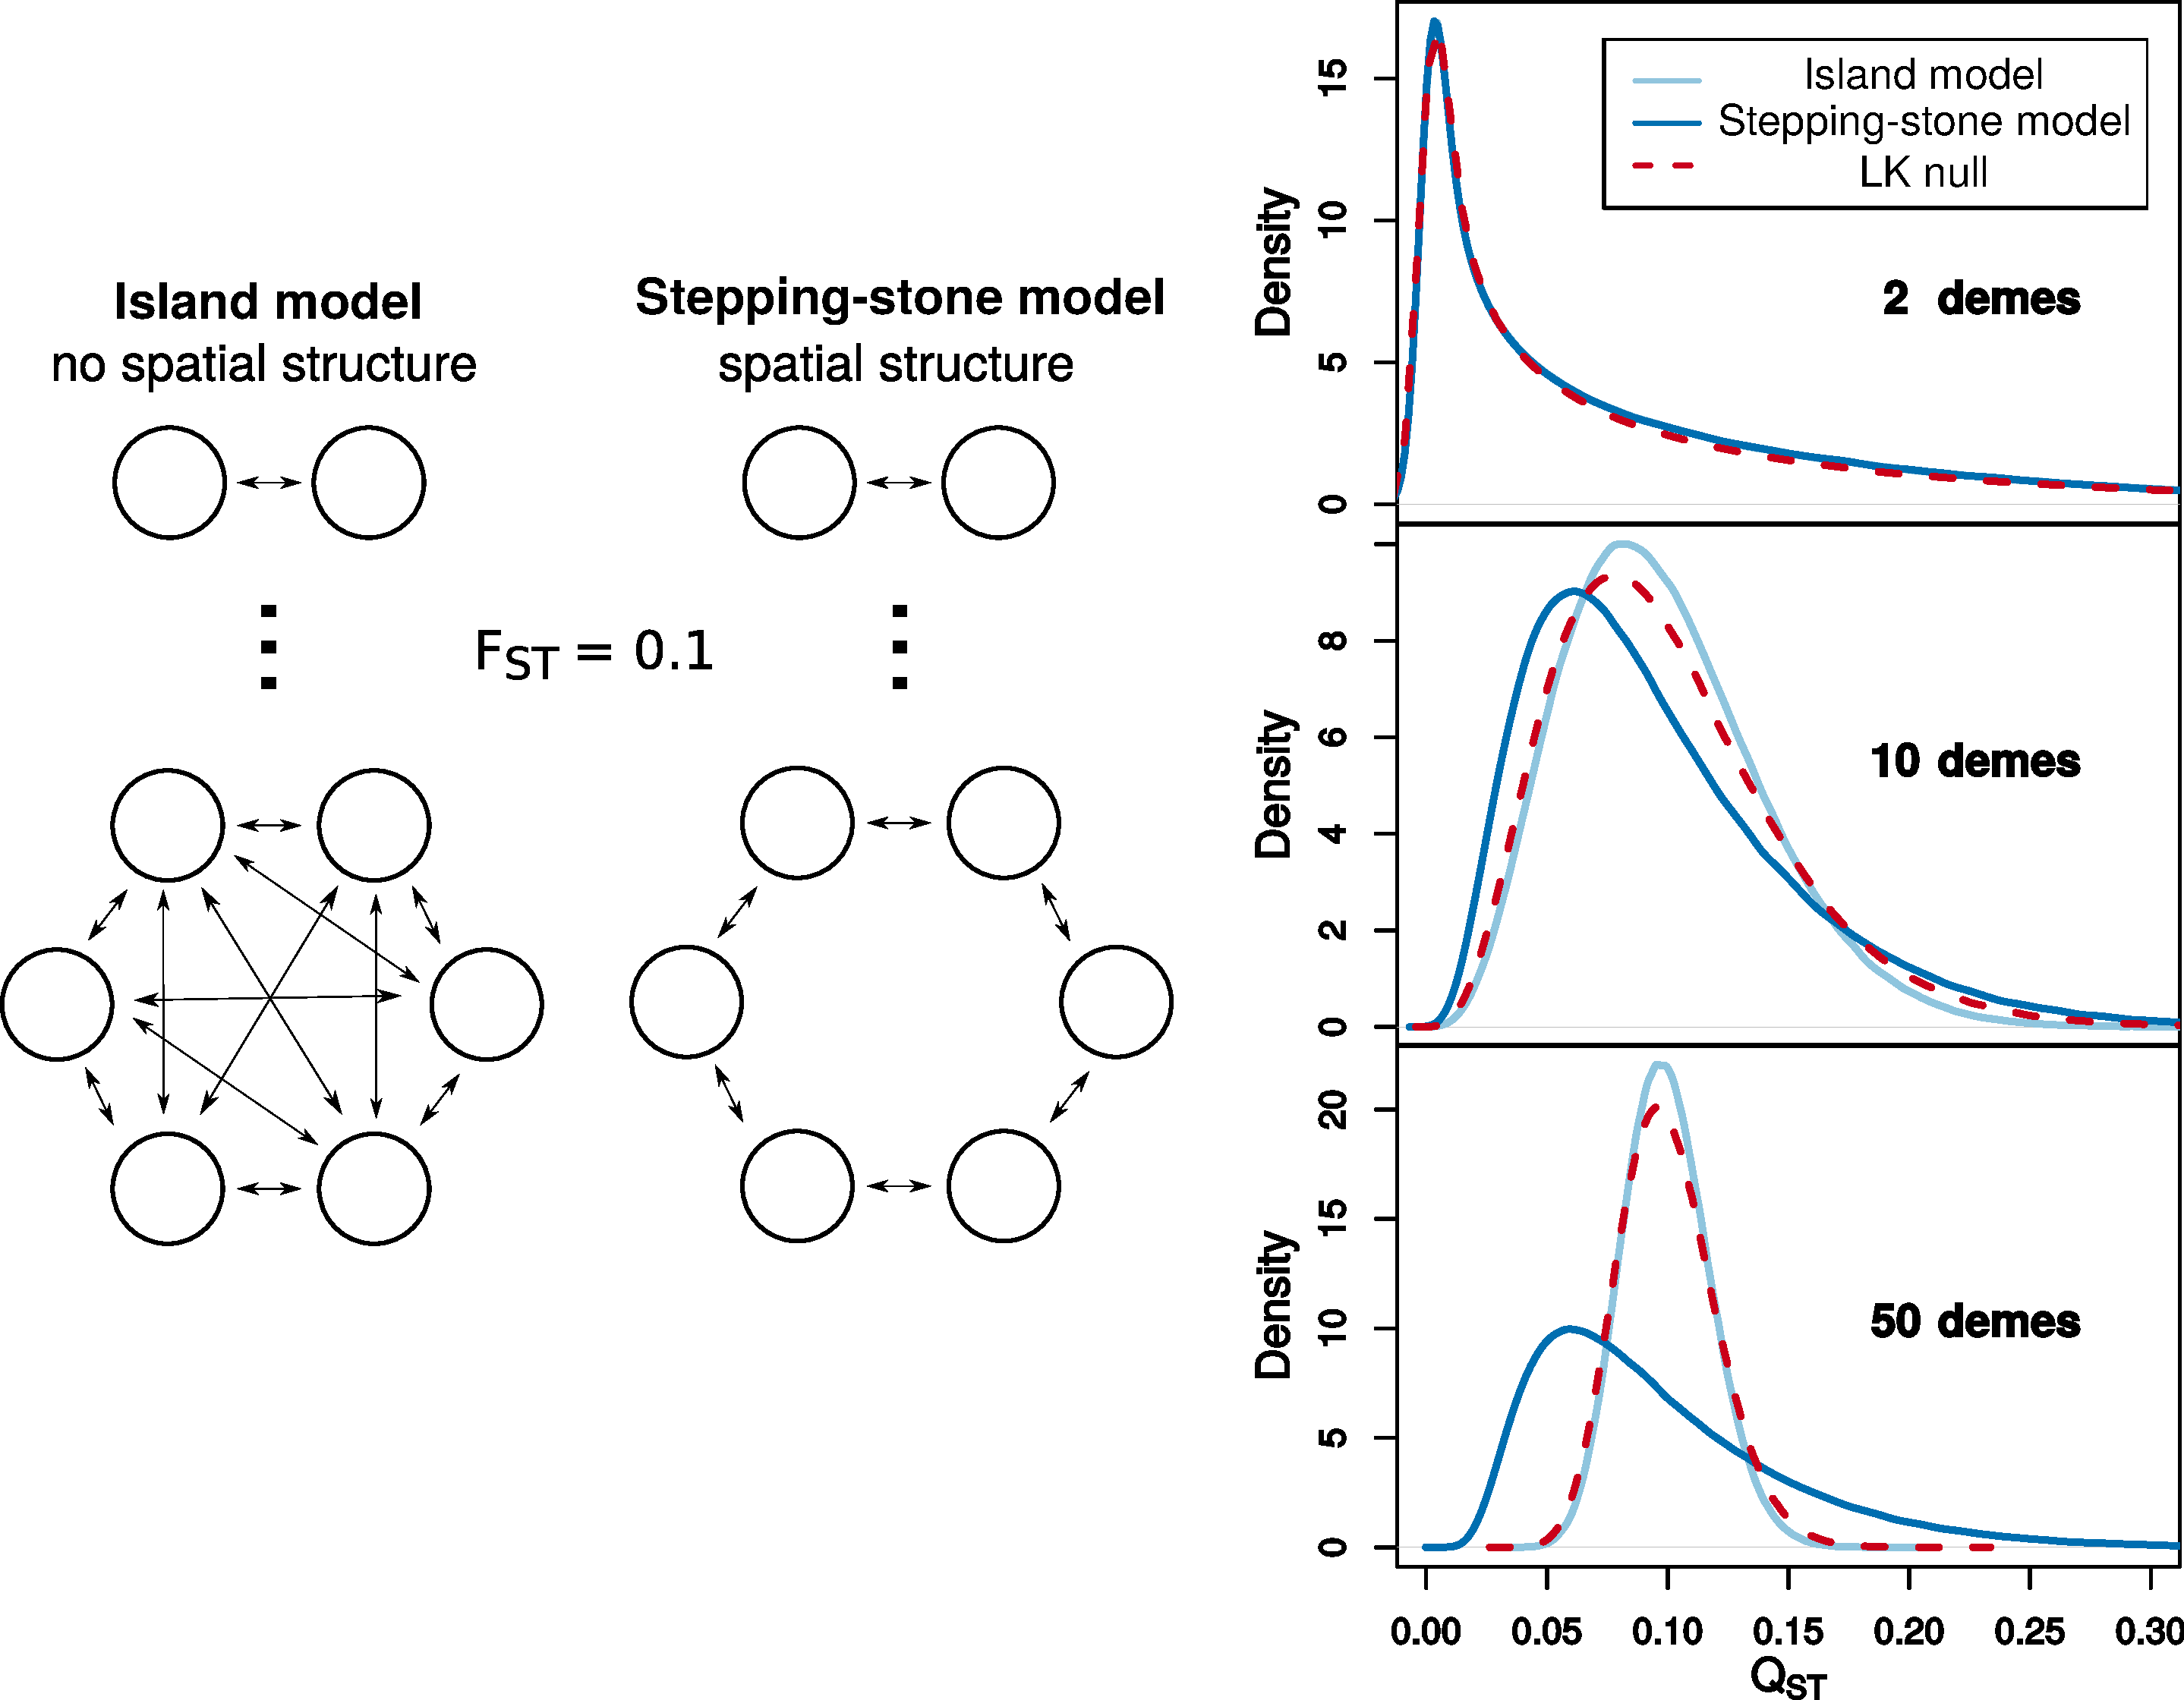
\includegraphics[width=0.95\textwidth]{./figures/pop_struct_combine_alt.pdf}
  \caption{ \textbf{A comparison of neutral sampling distributions for
      $Q_{ST}$ at the population level.} The Lewontin-Krakauer (LK) distribution for $Q_{ST}$ is
    compared to the null distribution in the infinitesimal limit in a case with
    (the stepping-stone model) and a case without (the island model) spatial
    structure. The case with no spatial structure assumes the migration rate is
    equal between all subpopulations, and the case with spatial structure
    arranges subpopulations in a ring with migration only between neighboring
    subpopulations. Migration rates and subpopulation sizes are all equal and
    are set such that $F_{ST}=0.1$ even as the number of subpopulations is
    increased \citep{Slatkin1991}. $Q_{ST}$ values for these models are
    simulated by drawing vectors from a multivariate normal distribution
    parameterized using the expected pairwise coalescence times given by
    \citep{Slatkin1991}. Under the LK distribution $Q_{ST}$ is distributed as
    $F_{ST}/(n_d - 1)$ times a chi-square distribution with $n_d - 1$ degrees of
    freedom ($Q_{ST}\sim F_{ST}\chi^2_{n_d - 1}/(n_d-1)$), where $n_d$ is the
    number of subpopulations. Vertical lines show the mean $Q_{ST}$ under the
    different null distributions. The mean $Q_{ST}$ values for the two normal
    models are nearly identical. Discordance between these lines and that for
    the LK distribution illustrates that $Q_{ST} \neq F_{ST}$. The neutral
    distributions for $Q_{ST}$ become increasingly different as the number of
    subpopulations over which the genetic divergence is spread increases.}
  \label{fig:qst_deme}
\end{figure}

\begin{figure}
  \centering
  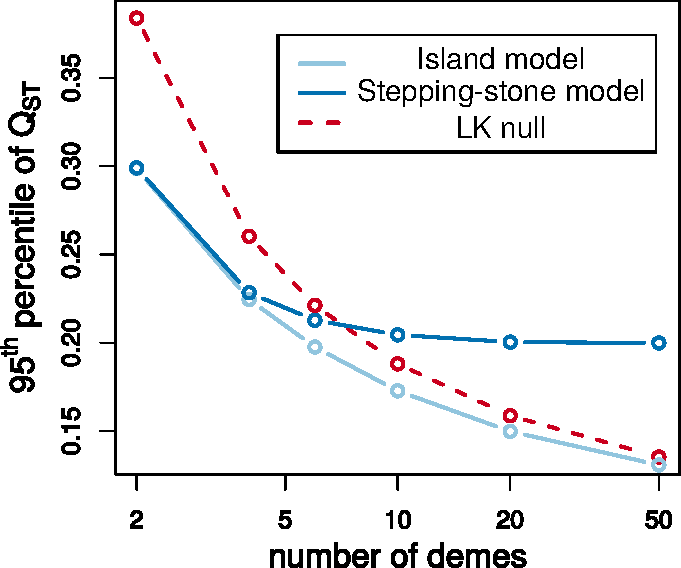
\includegraphics[width=0.5\textwidth]{./figures/qst_deme_percentile_nospace_alt.pdf}
  \caption{\textbf{Differences in the $95^{\mathrm{th}}$ percentile of different
      neutral sampling distributions for $Q_{ST}$ at the population level.} The
    Lewontin-Krakauer (LK) distribution is compared to neutral null
    distributions for structured populations with and without a spatial
    component using the multivariate normal model that arises in the
    infinitesimal limit.}
  \label{fig:qst_perc}
\end{figure}


To demonstrate the utility of the normal distribution arising in the
infinitesimal limit (equation \ref{eq:normcov}), we derive a simple procedure
for simulating from null distribution for the divergence between groups in
structured populations. A common way to quantify the divergence in trait values
between groups is $Q_{ST}$, defined as the variance between the group means
divided by the total variance in the population \citep{Spitze1993}. In a haploid
model, $Q_{ST} = \frac{V_{between}}{V_{between} + V_{within}}$, where
\begin{equation*}
  V_{between} = \frac{1}{K} \sum_i \left( \bar{Y}_i - \bar{Y} \right)^2
\end{equation*}
and
\begin{equation*}
  V_{within} = \frac{1}{\sum_k N_k} \sum_i \sum_j \left( Y_{i,j} - \bar{Y}_i \right)^2.
\end{equation*}
Here, $Y_{i,j}$ is the trait value of individual $j$ in population $i$, $K$ is
the number of subpopulations, and $N_k$ is the size of subpopulation $k$.

In the normal model, all $Y_{i,j}$ are normally distributed. Therefore,
$\bar{Y}_{i} - \bar{Y}$ and $Y_{i,j} - \bar{Y}_i$ are also normally distributed.
When population sizes are large, individual deviations from population means are
nearly uncorrelated, as are $V_{between}$ and $V_{within}$. $V_{within}$ is
nearly constant across evolutionary realizations and is equal to $\sum_k N_k
E[\mathcal{T}_{k,k}] / \sum_k N_k$ because the within population variances are
approximately uncorrelated and their variances are order $1/N_k$. While we do
not have an explicit form for the density function of the between-group
variance, we can simulate from its distribution by drawing a vector of
$\bar{Y}_{i} - \bar{Y}$ values from a multivariate normal distribution with mean
zero and with a covariance matrix whose element between populations $a$ and $b$
is
\begin{equation}
  \Cov[\bar{Y}_{a} - \bar{Y}, \bar{Y}_{b} - \bar{Y}] =
  \mu_2 \T (\E[\mathcal{T}_{a,\cdot}] + \E[\mathcal{T}_{b,\cdot}] -
  \E[\mathcal{T}_{\cdot,\cdot}] - \E[\mathcal{T}_{a,b}]).
\end{equation}
To simulate $Q_{ST}$ values we do not need to know $\mu_2$ or $\T$ because the
scale of the trait variance cancels in the $Q_{ST}$ ratio. Therefore, all that
is necessary to simulate from the null distribution of $Q_{ST}$ is to have
estimates of the expected coalescent time within and between populations. No
further information about the history or structure of the population is needed.
Since only the relative coalescent times matter it is also not necessary to
scale these estimates to units of years or generations using a mutation rate.

This procedure for simulating from the null distribution of $Q_{ST}$ could be
useful in testing whether an observed $Q_{ST}$ is unlikely under neutrality.
Current goodness-of-fit tests either compare $Q_{ST}$ to an empirical
distribution of $F_{ST}$ values or to a $\chi^2$ distribution
\citep{Leinonen2013}. In the second case, an identical distribution to that
developed by \citet{Lewontin1973} is used as the null distribution for $Q_{ST}$.
The $\chi^2$ testing procedure was suggested by \citet{Whitlock2009} and is
implemented in the program \textit{QstFstComp} \citep{Gilbert2015}. The
Lewontin-Krakauer (LK) distribution assumes independence between subpopulations
and provides a good approximation in populations without spatial structure, such
as in a symmetric island model of migration (Figure \ref{fig:qst_deme}). When
subpopulations are strongly correlated, such as in a one-dimensional
stepping-stone model of population structure, the LK distribution is a poor
approximation. Even when the distributions appear qualitatively similar, there
are substantial differences in tail probabilities (Figure \ref{fig:qst_perc}).

Nearly identical issues to these were raised with the LK test at the time of its
publishing \citep{Nei1975,Robertson1975}. However, while the neutral
distribution for $F_{ST}$ depends on the precise details of population structure
and history, the distribution of $Q_{ST}$ only depends on the set of within and
between subpopulation coalescence times. The point here is not that the LK
distribution is particularly bad, but rather that an improved neutral
distribution can be obtained using the normal model arising in the infinitesimal
limit. The neutral distribution described here is similar to the extension of
the LK test developed by \citet{Bonhomme2010} to account for the correlation
structure between subpopulations. The \citet{Bonhomme2010} method treats allele
frequencies as multivariate normal with covariance matrix parameterized by
coancestry coefficients. \citet{Ovaskainen2011} use a normal model similar to
that found in the infinitesimal limit here, but the covariance matrix is also
based on coancestry coefficients. When phenotypic and genetic divergence is
mostly driven by changes in allele frequency, the coalescent and coancestry
based models should be very similar. However, the coalescent model is ultimately
preferable since it is the correct null model at any scale of population
divergence in the infinitesimal limit. When only allele frequency data are
available, a coancestry model is the only option, but it is still better to
model variable levels of shared ancestry between populations than to use a
single value of $F_{ST}$.

Additionally, treating $Q_{ST}$ as a random variable lets us reexamine the
classic result in evolutionary quantitative genetics that $Q_{ST}=F_{ST}$
\citep{Whitlock1999}. $F_{ST}$, in this context, refers to a parameter of the
population. In particular, $F_{ST} = \frac{\bar{t} - \bar{t}_0}{\bar{t}}$, where
$\bar{t}$ is the expected coalescent time for two loci sampled at random from
the entire population and $\bar{t}_0$ is the expected coalescent time for two
loci sampled within a subpopulation \citep{Slatkin1991}. This value is constant
over realizations of the evolutionary process. $Q_{ST}$ can only refer to either
state of the population or to an estimate of this state. As shown above,
$Q_{ST}$, as a state of the population, varies across evolutionary realizations.
Thus, there is no sense in which $Q_{ST}$ can be defined as a constant parameter
in the way that $F_{ST}$ can. The expectation of $V_{between}$ is $\bar{t} -
\bar{t}_0$, and the expectation of $V_{within}$ is $\bar{t}_0$.
$\frac{\E[V_{between}]}{\E[V_{between}] + \E[V_{within}]}$ is equal to $F_{ST}$,
but due to Jensen's inequality, the expectation of this ratio ($\E[Q_{ST}]$) is
always less than $F_{ST}$.

%%% Local Variables:
%%% TeX-master: "quant_gen_manu.tex"
%%% End:
